\chapter{Methodology and Results Interpretation}
\label{chap:methodology-results-interpretation}

\section{Data and Empirical Strategy}
\label{sec:data-empirical-strategy}

We study the association between domestic monetary conditions and FDI net inflows in an unbalanced ASEAN-oriented panel over 2000--2023. FDI net inflows (\% of GDP) is the dependent variable. Broad money growth is used as the liquidity proxy, while the real interest rate proxies the cost of capital. Controls include GDP growth, log GDP per capita, trade openness (\% of GDP), exchange-rate depreciation, inflation, and Regulatory Quality.

The empirical sequence is summarized as follows:
\begin{itemize}
    \item \textbf{Spec 1:} baseline controls only.
    \item \textbf{Spec 2:} baseline controls plus the real interest rate.
    \item \textbf{Spec 3:} baseline controls plus Regulatory Quality.
    \item \textbf{Spec 4:} the full static specification with the real interest rate and Regulatory Quality.
    \item \textbf{Spec 5:} the full model plus lagged FDI, estimated with two-step System GMM and Windmeijer-corrected standard errors.
\end{itemize}

The static models report country-clustered standard errors and include country and year effects; Spec 1 is estimated with random effects, while Specs 2--4 use fixed effects. The dynamic specification uses year fixed effects and reports standard GMM diagnostics.

The preferred static specification can be written as:
\begin{equation}
    FDI_{it} = \beta_1 BM_{it} + \beta_2 IR_{it}^{(k)} + \boldsymbol{\gamma}'\mathbf{X}_{it} + \alpha_i + \lambda_t + \varepsilon_{it},
\end{equation}
where $\alpha_i$ and $\lambda_t$ are country and year effects.

\section{Main Results}
\label{sec:main-results}

\begin{table}[htbp]
\centering
\caption{Two-way fixed-effects regression results with Driscoll–Kraay standard errors}
\label{tab:main-regression-results}
\begin{threeparttable}
\scriptsize
\resizebox{\textwidth}{!}{%
\begin{tabular}{lccccccccc}
\toprule
 & \multicolumn{5}{c}{Panel A: Headline Models} & \multicolumn{4}{c}{Panel B: Extended Models} \\
\cmidrule(lr){2-6} \cmidrule(lr){7-10}
 & M1 & M2 & M3 & M4 & M5 & M6a & M6b & M7a & M7b \\
\midrule
Broad money growth (annual \%) & 0.0460* & 0.0451 & 0.1223** & 0.0351 & 0.0627* & 0.0446 & 0.0422 & 0.0494 & 0.0453 \\
 & (0.0277) & (0.0388) & (0.0572) & (0.0426) & (0.0360) & (0.0395) & (0.0386) & (0.0432) & (0.0392) \\
Deposit interest rate (\%) &  & 0.0922 & 0.1274 &  &  &  & 0.0883 &  & 0.0887 \\
 &  & (0.1242) & (0.1521) &  &  &  & (0.1217) &  & (0.1700) \\
Real interest rate (\%) &  &  &  & -0.3225 &  & 0.0836 &  & 0.0743 &  \\
 &  &  &  & (0.2370) &  & (0.1128) &  & (0.1380) &  \\
Lending interest rate (\%) &  &  &  &  & 0.2500 &  &  &  &  \\
 &  &  &  &  & (0.1738) &  &  &  &  \\
Tourism arrivals (Log) &  &  &  &  &  & -0.5474 & -0.5260 &  &  \\
 &  &  &  &  &  & (0.6736) & (0.6588) &  &  \\
Human capital index &  &  &  &  &  &  &  & 0.7949 & 0.1646 \\
 &  &  &  &  &  &  &  & (3.2223) & (3.2596) \\
Trade (\% GDP) & -0.0014 & -0.0154 & -0.0170 & -0.0126 & -0.0182 & -0.0134 & -0.0120 & -0.0165 & -0.0153 \\
 & (0.0123) & (0.0175) & (0.0198) & (0.0184) & (0.0167) & (0.0188) & (0.0195) & (0.0174) & (0.0178) \\
Inflation (\%) & -0.0195 & 0.0017 & -0.0322 & -0.2957 & -0.0200 & 0.0785 & 0.0012 & 0.0695 & 0.0017 \\
 & (0.0576) & (0.0441) & (0.0485) & (0.1988) & (0.0396) & (0.1274) & (0.0447) & (0.1534) & (0.0443) \\
Log GDP per capita & 0.2059 & 0.9642* & 1.1131 & -0.9521 & 1.8815*** & 1.2607** & 0.8889 & 1.2495** & 0.9459 \\
 & (1.5284) & (0.5560) & (0.8672) & (1.2826) & (0.5928) & (0.5675) & (0.5750) & (0.5319) & (0.6209) \\
Exchange-rate depreciation (\%) & 0.0153 & 0.0539 & 0.0585 & 0.0801* & 0.0624 & 0.0637* & 0.0560 & 0.0618* & 0.0540 \\
 & (0.0272) & (0.0413) & (0.0469) & (0.0427) & (0.0384) & (0.0368) & (0.0425) & (0.0344) & (0.0407) \\
Observations & 209 & 149 & 145 & 164 & 151 & 151 & 149 & 151 & 149 \\
Countries & 10 & 7 & 7 & 8 & 7 & 7 & 7 & 7 & 7 \\
Within $R^2$ & 0.0305 & 0.0655 & 0.0883 & 0.0352 & 0.0535 & 0.0387 & 0.0393 & 0.0476 & 0.0653 \\
Slope-adj. $R^2$ & 0.0066 & 0.0260 & 0.0486 & -0.0017 & 0.0141 & -0.0084 & -0.0084 & 0.0010 & 0.0189 \\
Max VIF & 5.27 & 7.18 & 7.26 & 9.74 & 12.62 & 667.94 & 582.07 & 179.50 & 207.32 \\
Pesaran CD $p$ & 0.0765 & 0.3760 & 0.6651 & 0.0539 & 0.3604 & 0.5234 & 0.4032 & 0.4543 & 0.3713 \\
\bottomrule
\end{tabular}
}
\begin{tablenotes}[flushleft]
\footnotesize
\item The dependent variable is FDI net inflows (\% of GDP). All columns use two-way fixed effects with country and year effects and Driscoll--Kraay standard errors (Bartlett kernel). Standard errors in parentheses. *, **, *** denote significance at 10\%, 5\%, 1\% levels. Panel A: headline models. Panel B: robustness models adding tourism arrivals (M6a, M6b) or the human capital index (M7a, M7b) to the M4 and M2 baselines respectively. Samples vary by model due to unbalanced panel coverage.
\end{tablenotes}
\end{threeparttable}
\end{table}

Across the static models in Panel A, broad money growth is positive and statistically significant in every specification, which is the clearest evidence in support of a liquidity channel. The real interest rate is positive and significant in Specs 2 and 4, so the data do not support a stable negative cost-of-capital effect. GDP growth and log GDP per capita are often positive and significant, while trade openness and exchange-rate depreciation are mostly imprecise. Inflation is positive and significant in the full static model.

In the dynamic System GMM estimate, lagged FDI is negative and significant, Regulatory Quality is positive and significant, and broad money growth is not statistically distinguishable from zero. That result should be interpreted cautiously because the AR(2) test rejects the null of no second-order serial correlation (\(p=0.0002\)).

\section{Limitations}
\label{sec:limitations}

Three caveats shape interpretation. (1) Samples vary by specification, so coefficients are not directly comparable across all models. (2) The dynamic specification is diagnostically fragile because of the AR(2) rejection. (3) The static estimates explain only a modest share of within-country variation, so the safest reading is associational rather than causal. The most defensible conclusion is that broad money growth is the most robust correlate of FDI inflows, while interest-rate and institutional effects are less stable and model-dependent.

\section*{Appendix}
\label{app:appendix}

\subsection{Summary Statistics}
\label{app:summary-stats}

Table~\ref{tab:descriptive-coverage} presents descriptive statistics for the processed panel. FDI inflows average 4.9\% of GDP but are highly dispersed (SD 6.2), ranging from $-16.2$ to $32.6$. Transactional variables (trade, FDI) and monetary aggregates exhibit substantial cross-country variation. Coverage varies: broad money is observed in 240 country-years, while lending rates are available in only 192 (27\% missing).

\begin{table}[htbp]
\centering
\caption{Descriptive statistics and data coverage for the processed panel (2000--2023)}
\label{tab:descriptive-coverage}
\begin{threeparttable}
\scriptsize
\resizebox{\textwidth}{!}{%
\begin{tabular}{lrrrrrl}
\toprule
Variable & N & Mean & SD & Min & Max & Missing \\\midrule
FDI (\% GDP) & 260 & 4.918 & 6.170 & -16.205 & 32.596 & 1.5\% \\
Broad money growth (annual \%) & 240 & 14.310 & 11.819 & -11.930 & 61.836 & 9.1\% \\
Deposit interest rate (\%) & 213 & 4.080 & 3.560 & 0.122 & 15.502 & 19.3\% \\
Real interest rate (\%) & 205 & 4.858 & 8.252 & -30.123 & 41.294 & 22.3\% \\
Lending interest rate (\%) & 192 & 9.783 & 6.392 & 3.060 & 32.000 & 27.3\% \\
Inflation, GDP deflator (\%) & 264 & 5.298 & 8.235 & -21.739 & 59.080 & 0.0\% \\
Trade (\% GDP) & 240 & 131.923 & 85.767 & 32.972 & 437.327 & 9.1\% \\
Log GDP per capita & 264 & 24.719 & 2.019 & 19.721 & 27.947 & 0.0\% \\
Exchange-rate depreciation (\%) & 253 & 2.700 & 30.527 & -13.362 & 476.795 & 4.2\% \\
Tourism arrivals (Log) & 240 & 15.258 & 1.150 & 12.938 & 17.502 & 9.1\% \\
Human capital index & 240 & 2.383 & 0.476 & 1.516 & 3.399 & 9.1\% \\
\bottomrule
\end{tabular}
}
\begin{tablenotes}[flushleft]
\footnotesize
\item N = country-year observations. The panel is unbalanced (max 264, min 192 per variable). FDI is expressed as a percentage of GDP. Monetary proxies have the narrowest coverage (lending rate: 192 obs). See the country-level audit tables for structural gaps.
\end{tablenotes}
\end{threeparttable}
\end{table}

\begin{figure}[htbp]
\centering
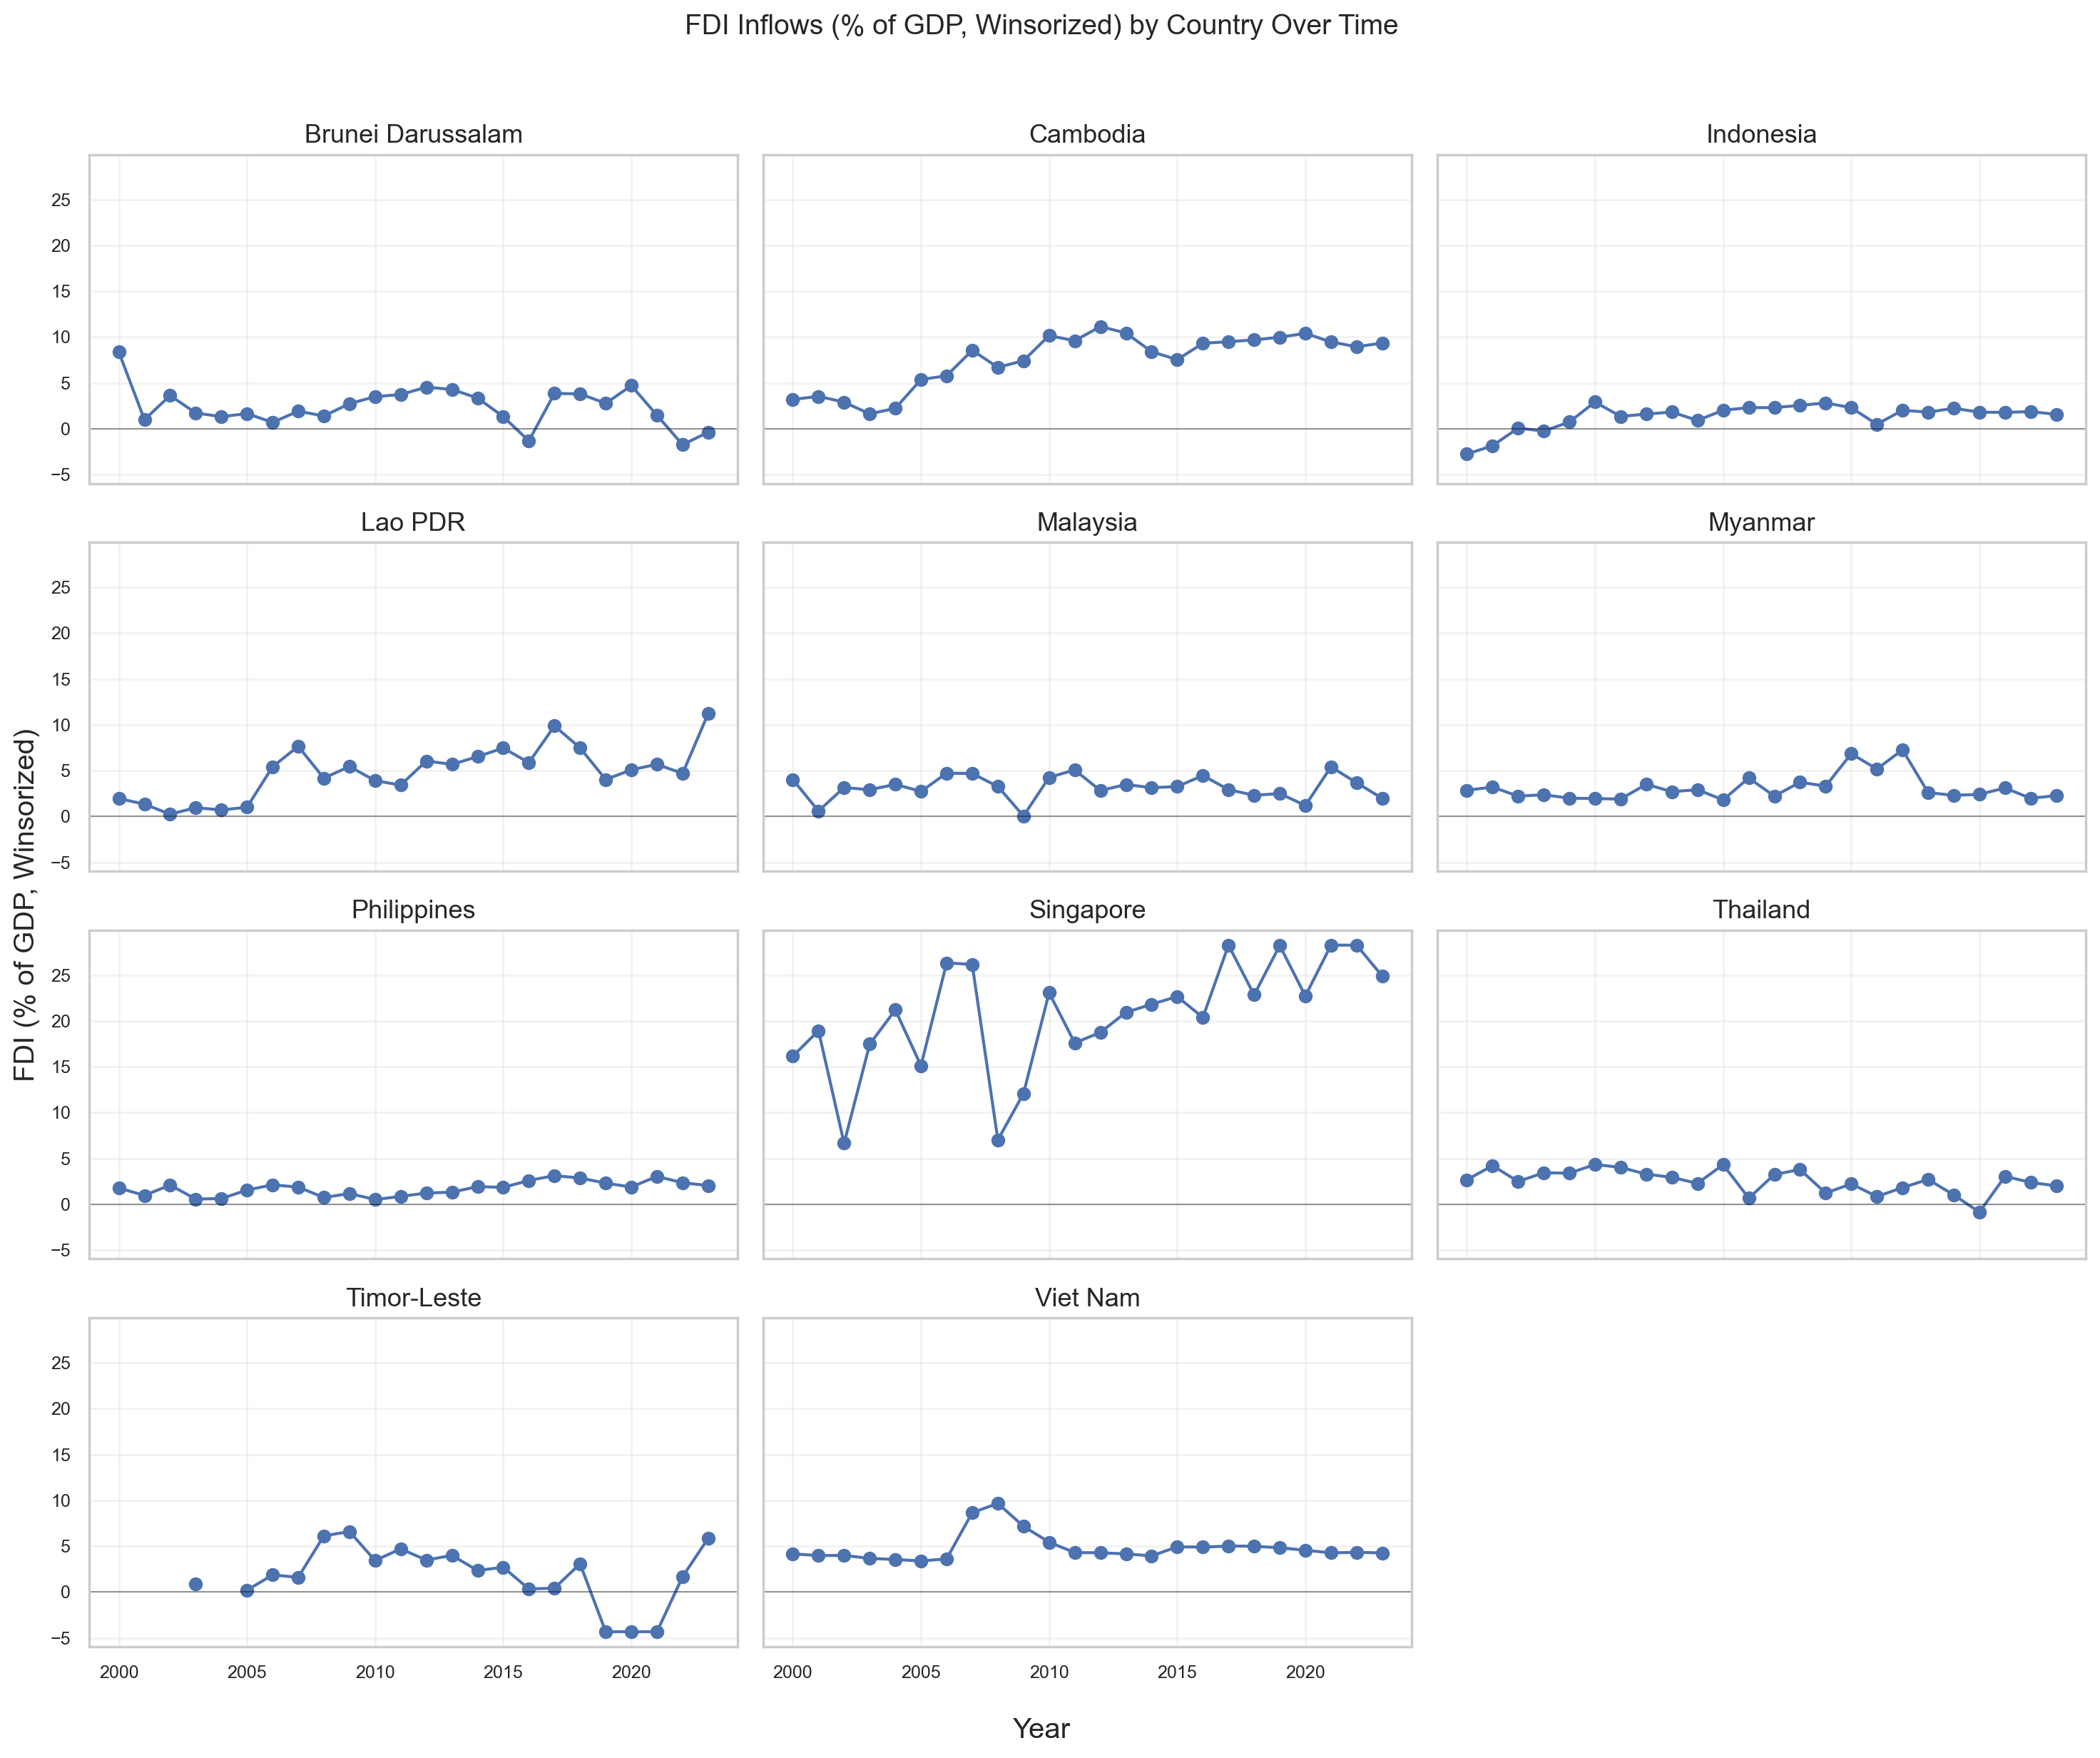
\includegraphics[width=\textwidth]{assets/small_multiples_country_fdi_trends.png}
\caption{FDI net inflows (\% of GDP) by country, 2000--2023. Country-level time series reveal substantial heterogeneity in levels and trends across ASEAN-oriented economies. Singapore's structurally high FDI-to-GDP ratio reflects its role as a regional financial hub.}
\label{fig:fdi-country-trends}
\end{figure}

\begin{figure}[htbp]
\centering
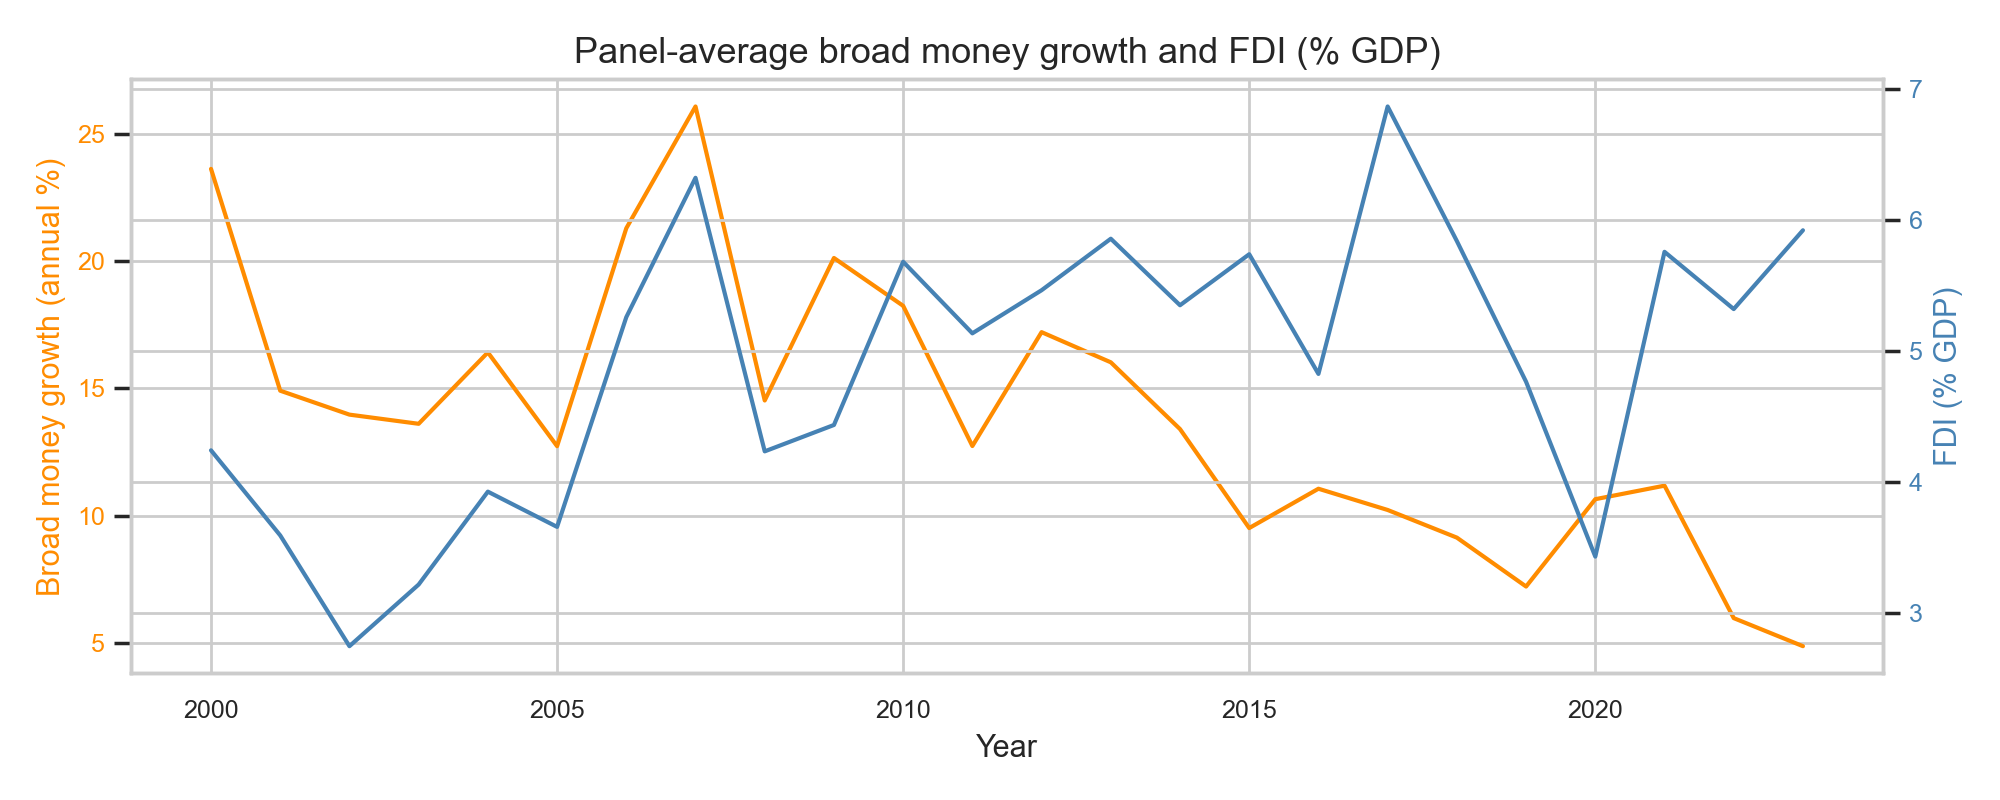
\includegraphics[width=\textwidth]{assets/yearly_broad_money_growth_and_fdi_trend.png}
\caption{Yearly cross-country average of broad money growth and FDI net inflows. Both series show a co-movement pattern consistent with a liquidity channel, particularly during the post-GFC period (2010--2015).}
\label{fig:trends}
\end{figure}

\subsection{Univariate Distributions}
\label{app:univariate}

\begin{figure}[htbp]
\centering
\begin{subfigure}[b]{0.32\textwidth}
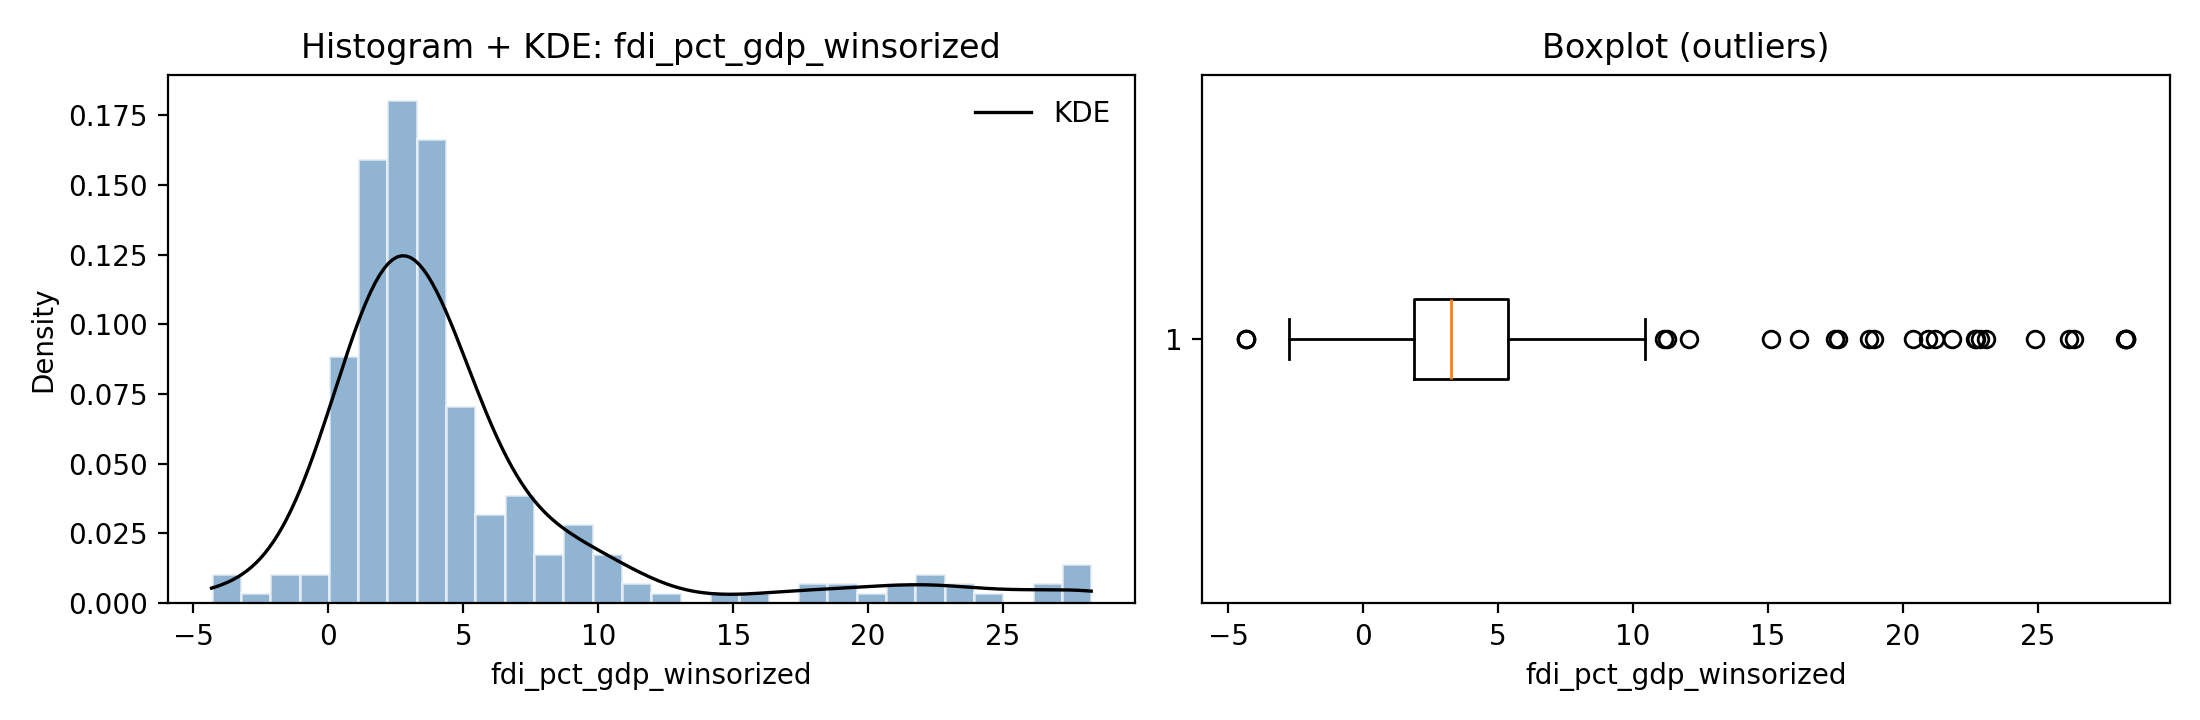
\includegraphics[width=\textwidth]{assets/univariate_dist__fdi_pct_gdp_winsorized.png}
\caption{FDI (\% GDP)}
\end{subfigure}
\begin{subfigure}[b]{0.32\textwidth}
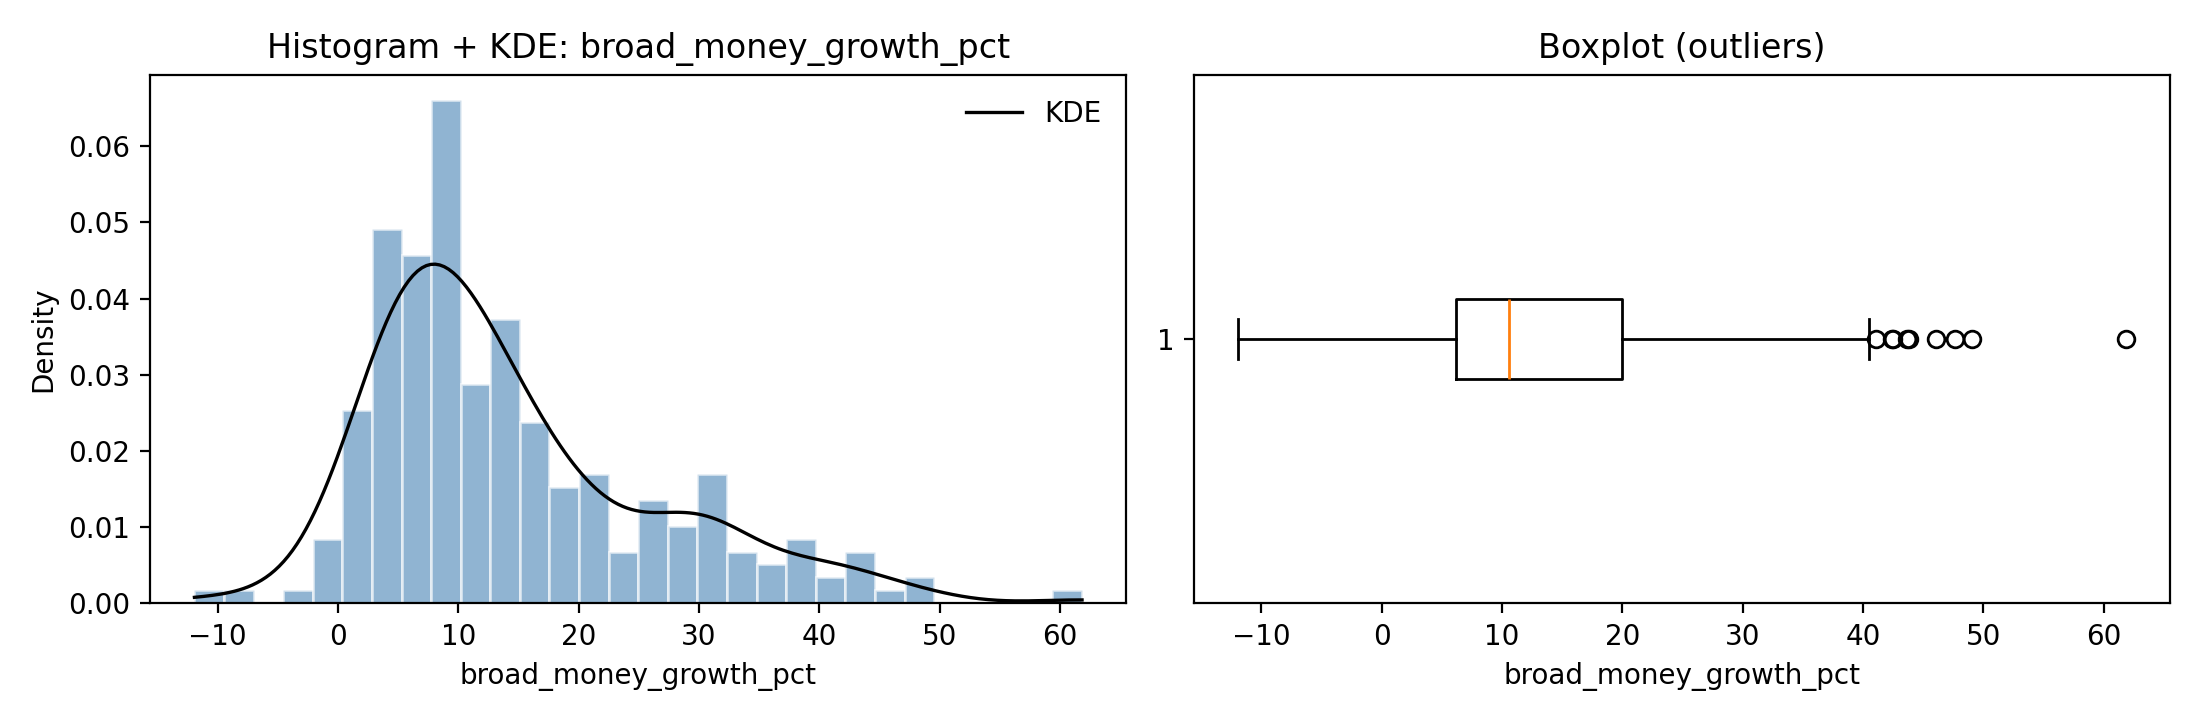
\includegraphics[width=\textwidth]{assets/univariate_dist__broad_money_growth_pct.png}
\caption{Broad money growth}
\end{subfigure}
\begin{subfigure}[b]{0.32\textwidth}
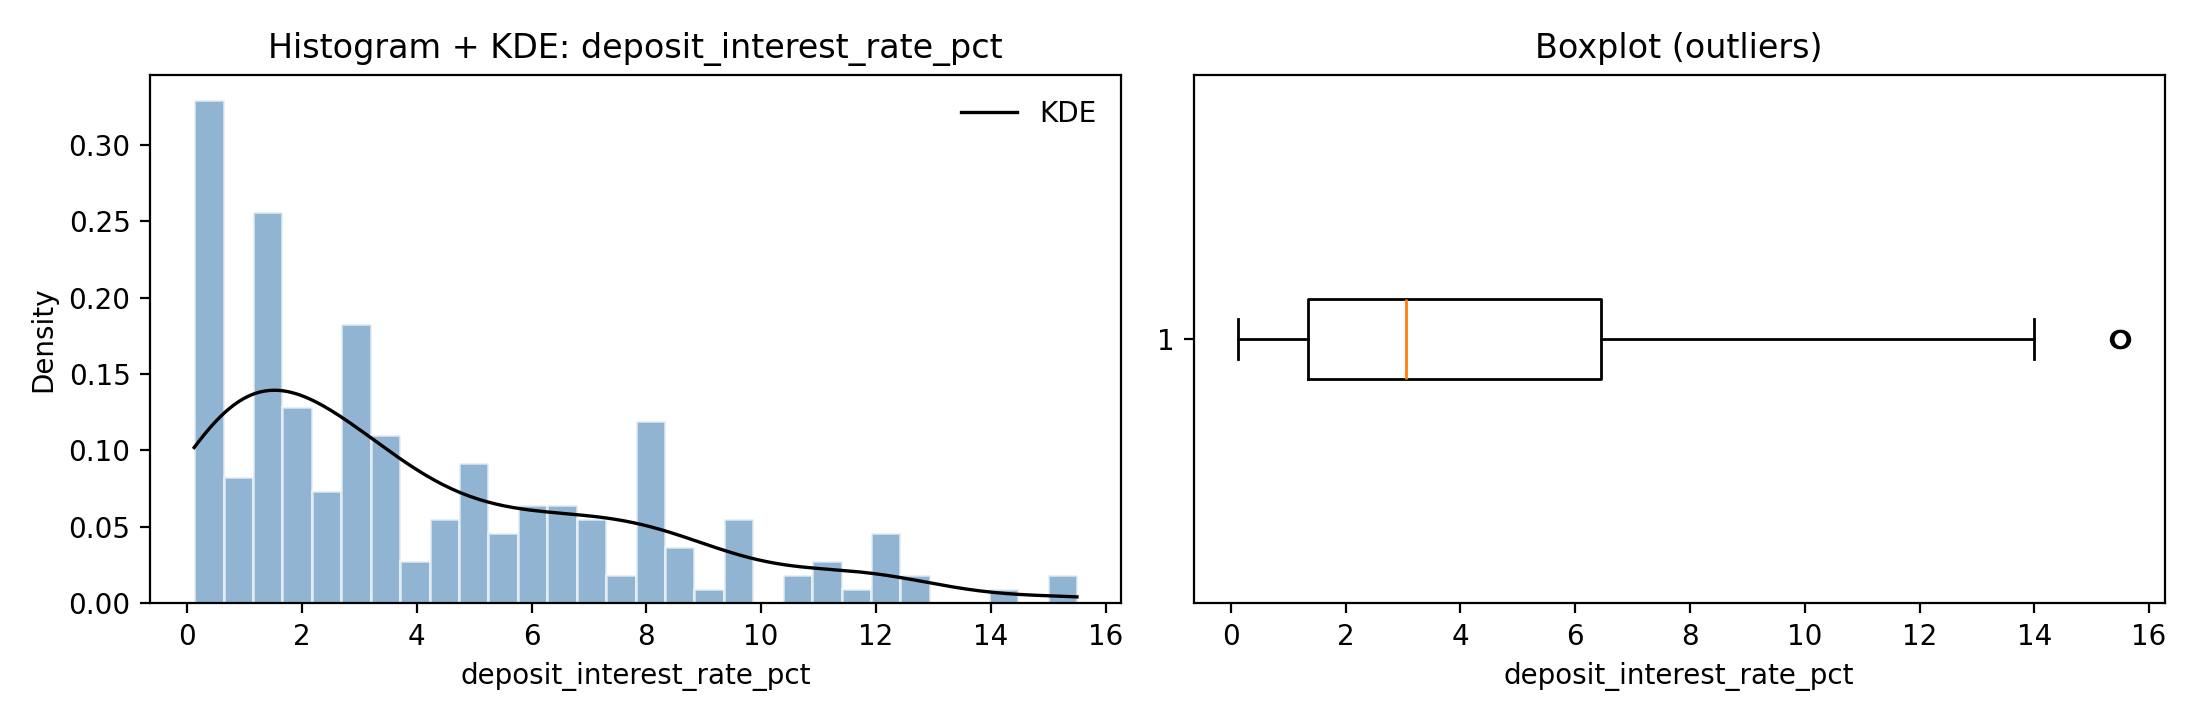
\includegraphics[width=\textwidth]{assets/univariate_dist__deposit_interest_rate_pct.png}
\caption{Deposit interest rate}
\end{subfigure}
\begin{subfigure}[b]{0.32\textwidth}
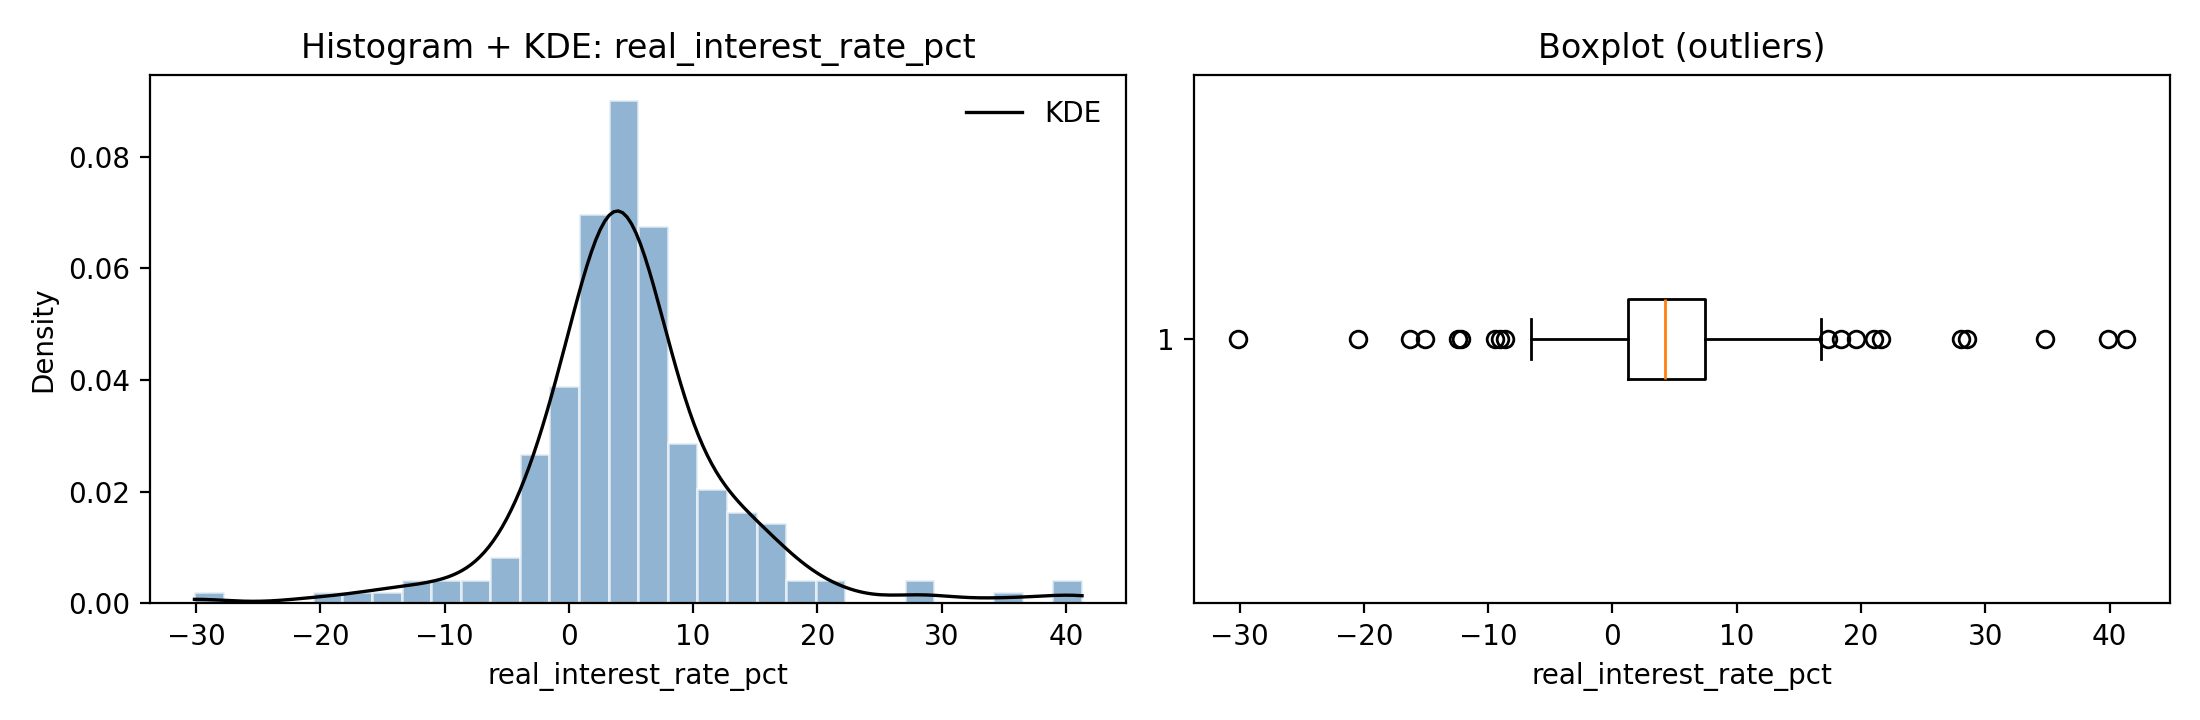
\includegraphics[width=\textwidth]{assets/univariate_dist__real_interest_rate_pct.png}
\caption{Real interest rate}
\end{subfigure}
\begin{subfigure}[b]{0.32\textwidth}
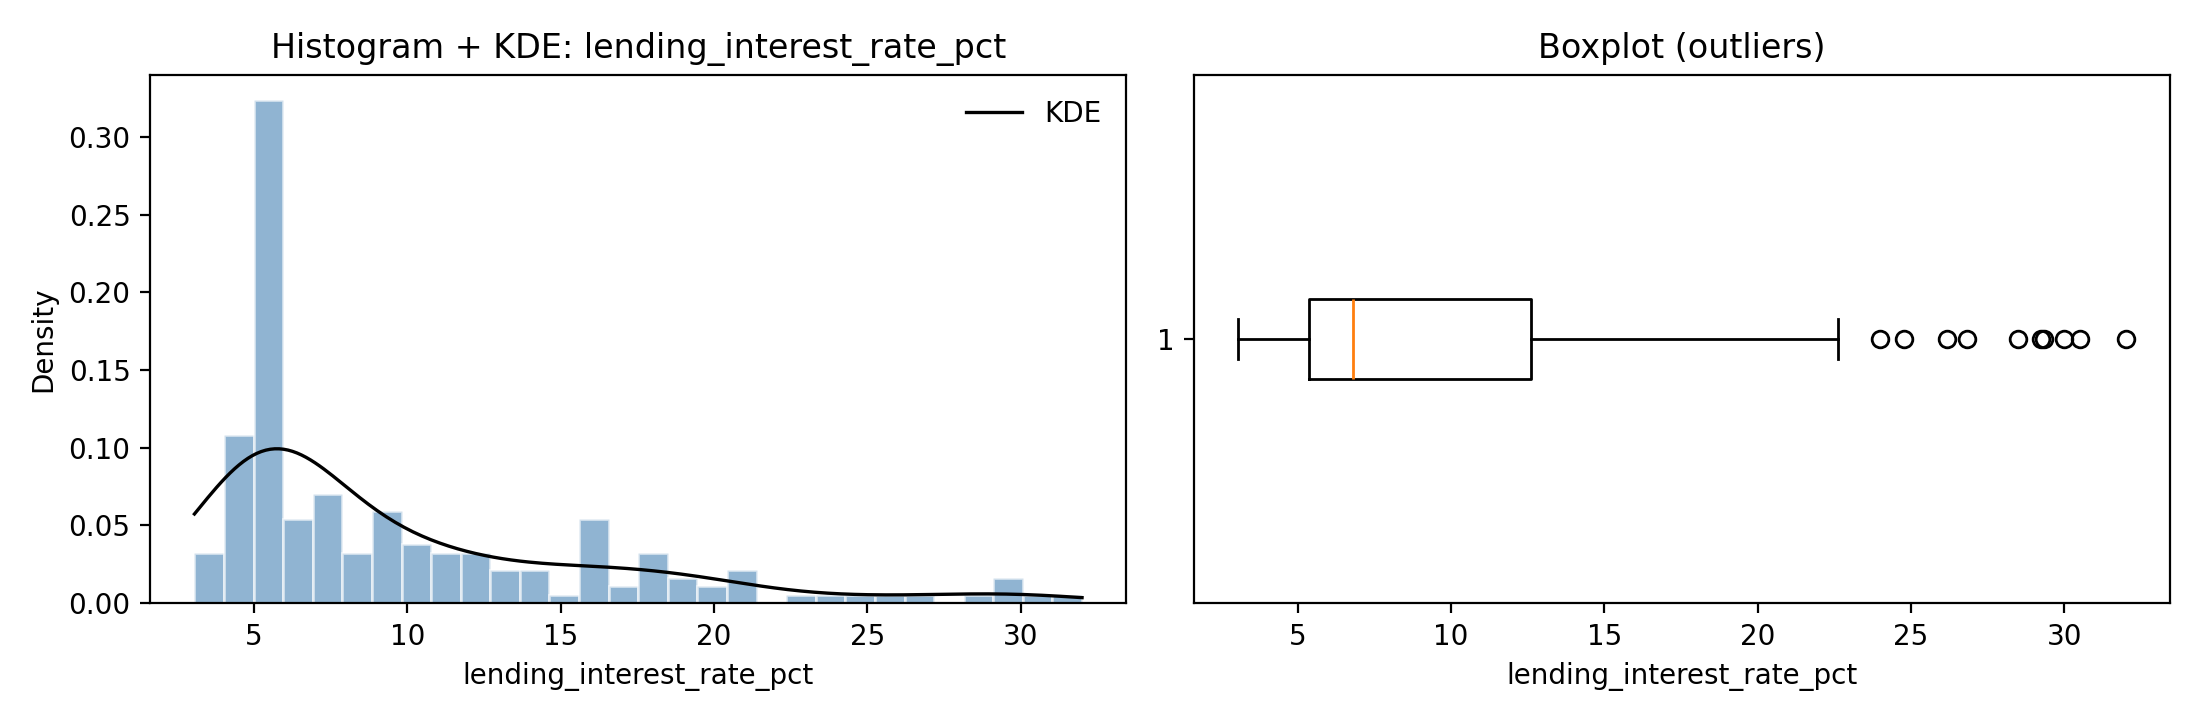
\includegraphics[width=\textwidth]{assets/univariate_dist__lending_interest_rate_pct.png}
\caption{Lending interest rate}
\end{subfigure}
\begin{subfigure}[b]{0.32\textwidth}
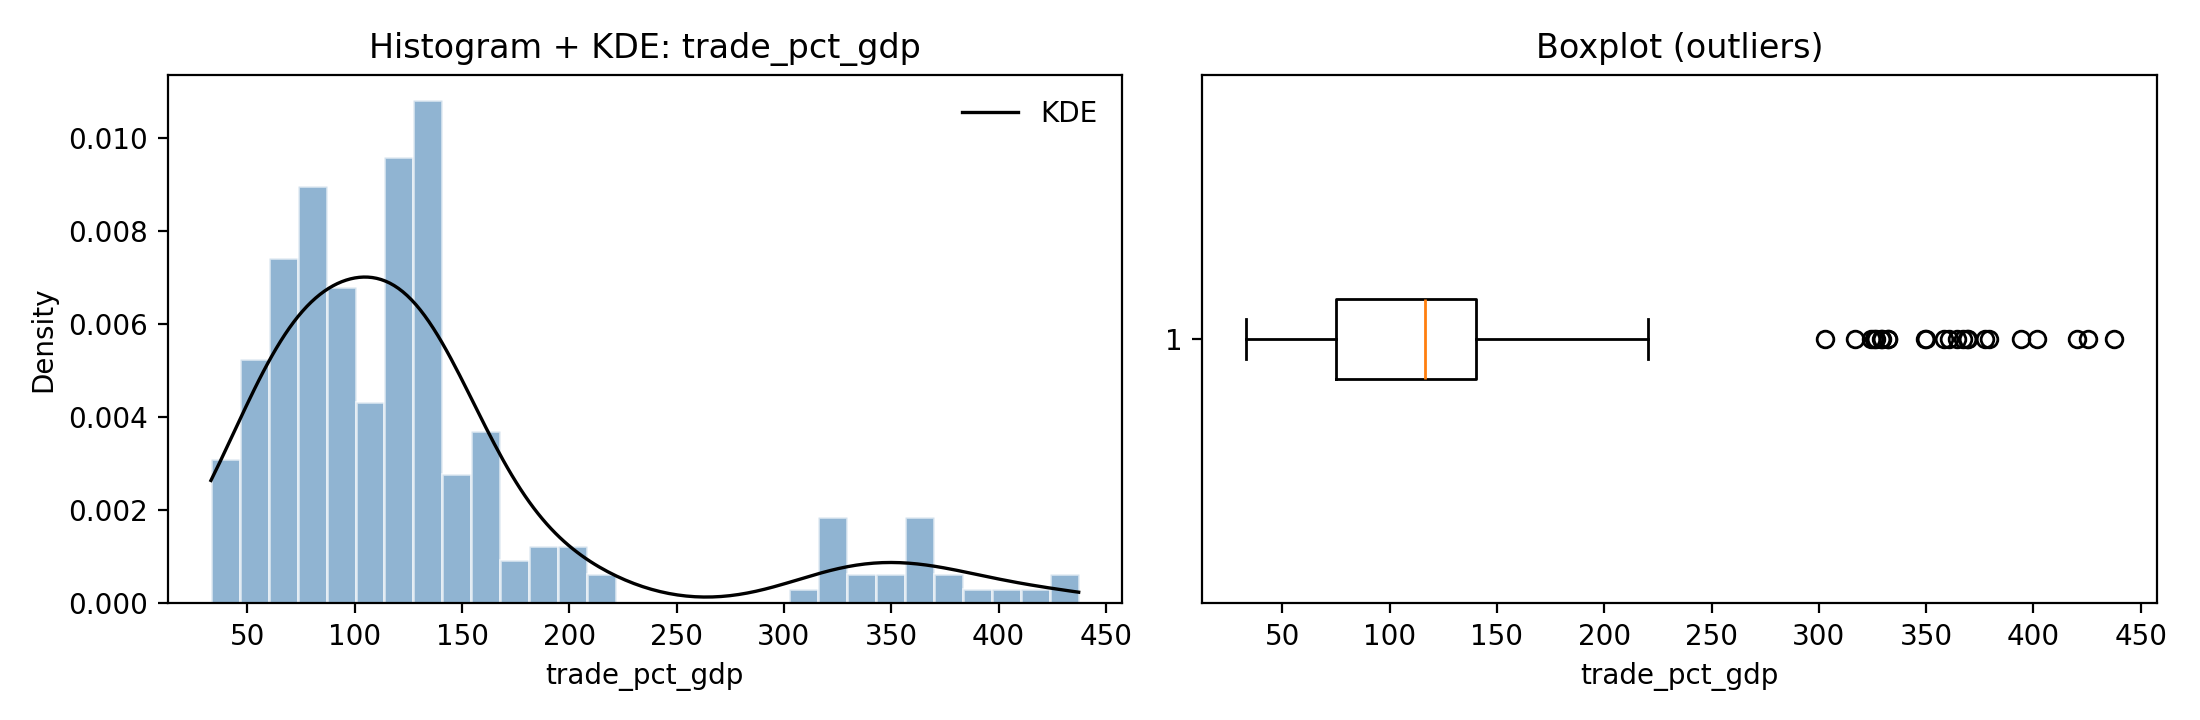
\includegraphics[width=\textwidth]{assets/univariate_dist__trade_pct_gdp.png}
\caption{Trade (\% GDP)}
\end{subfigure}
\caption{Distribution of key variables in the analytical panel. The monetary proxies (broad money, interest rates) and macro controls exhibit right-skewness and substantial dispersion, motivating the use of robust covariance estimation.}
\label{fig:univariate}
\end{figure}

\subsection{Bivariate Relationships}
\label{app:bivariate}

\begin{figure}[htbp]
\centering
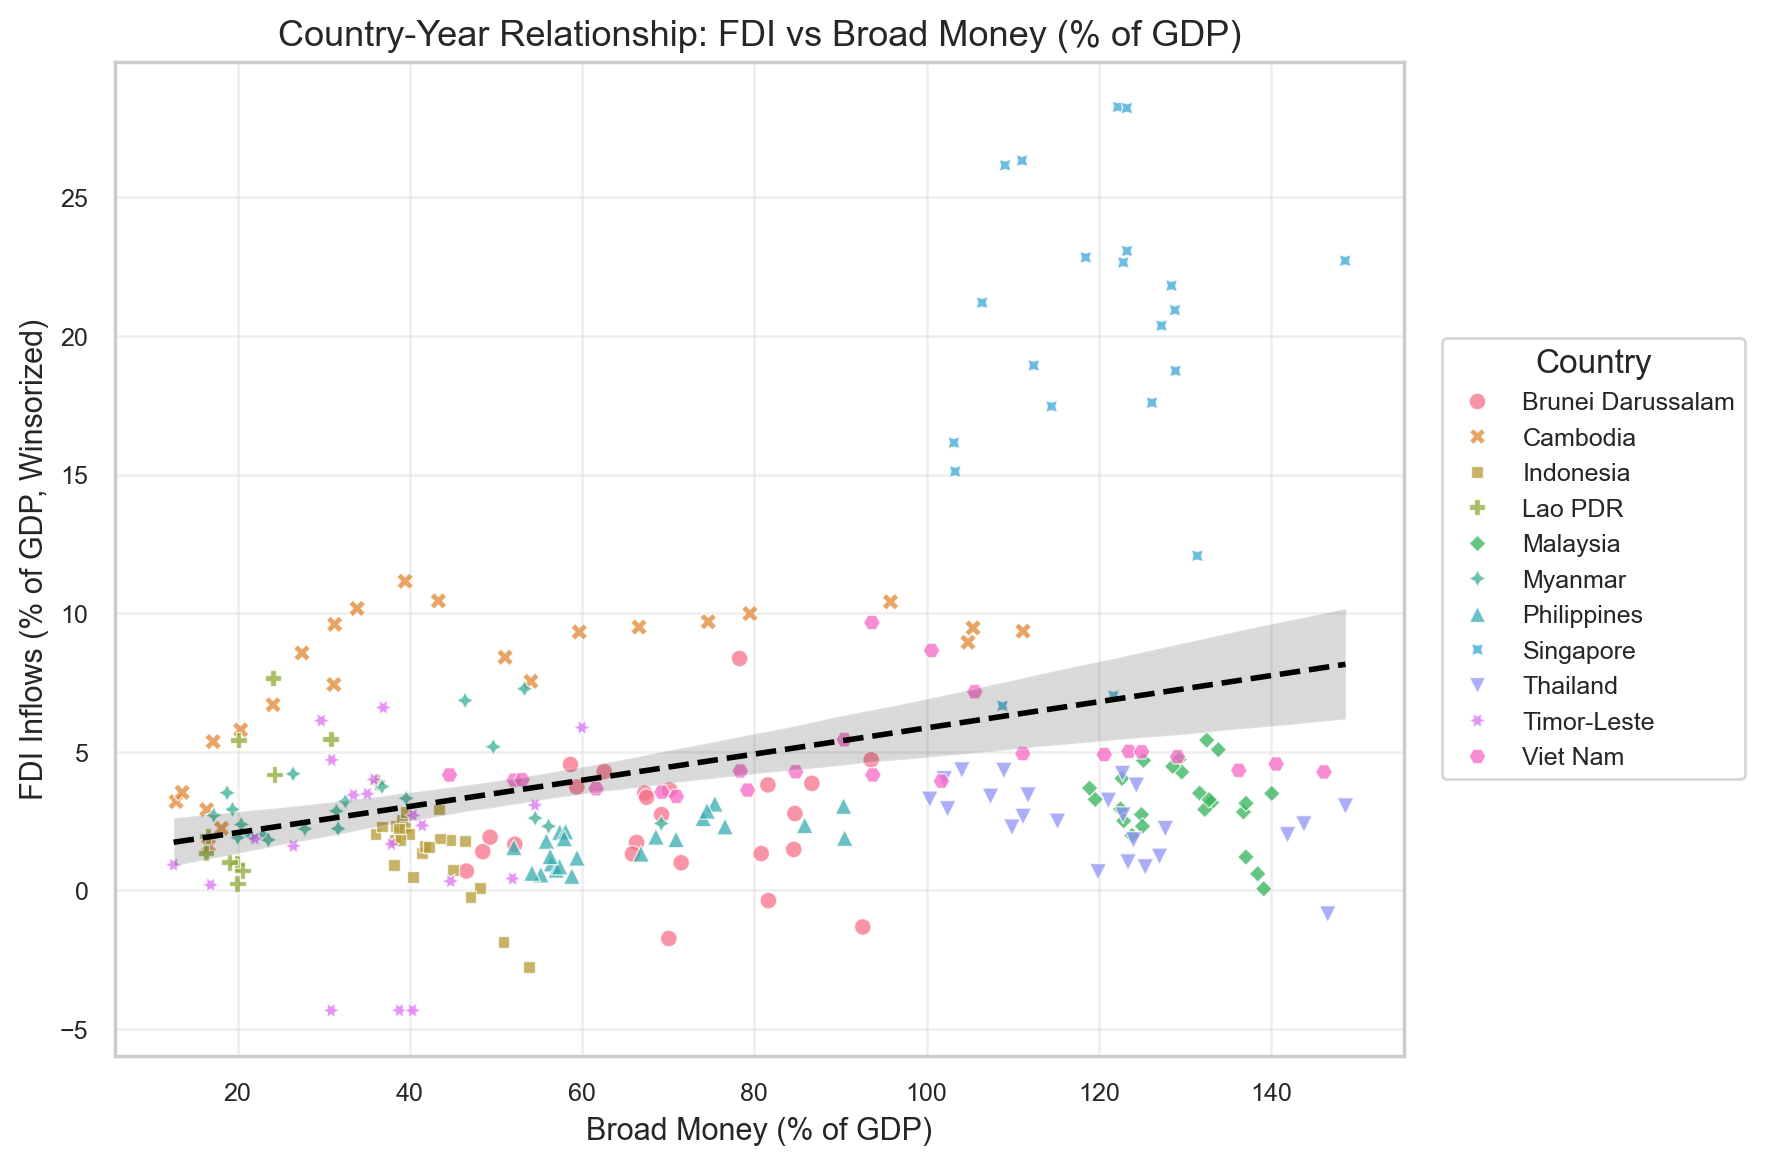
\includegraphics[width=0.75\textwidth]{assets/scatter_country_year_broad_money_fdi.png}
\caption{Broad money growth vs.\ FDI net inflows by country-year. The unconditional relationship is flat, consistent with the weak FE-DK coefficients in the main regression table.}
\label{fig:bivariate-bm-fdi}
\end{figure}

\begin{figure}[htbp]
\centering
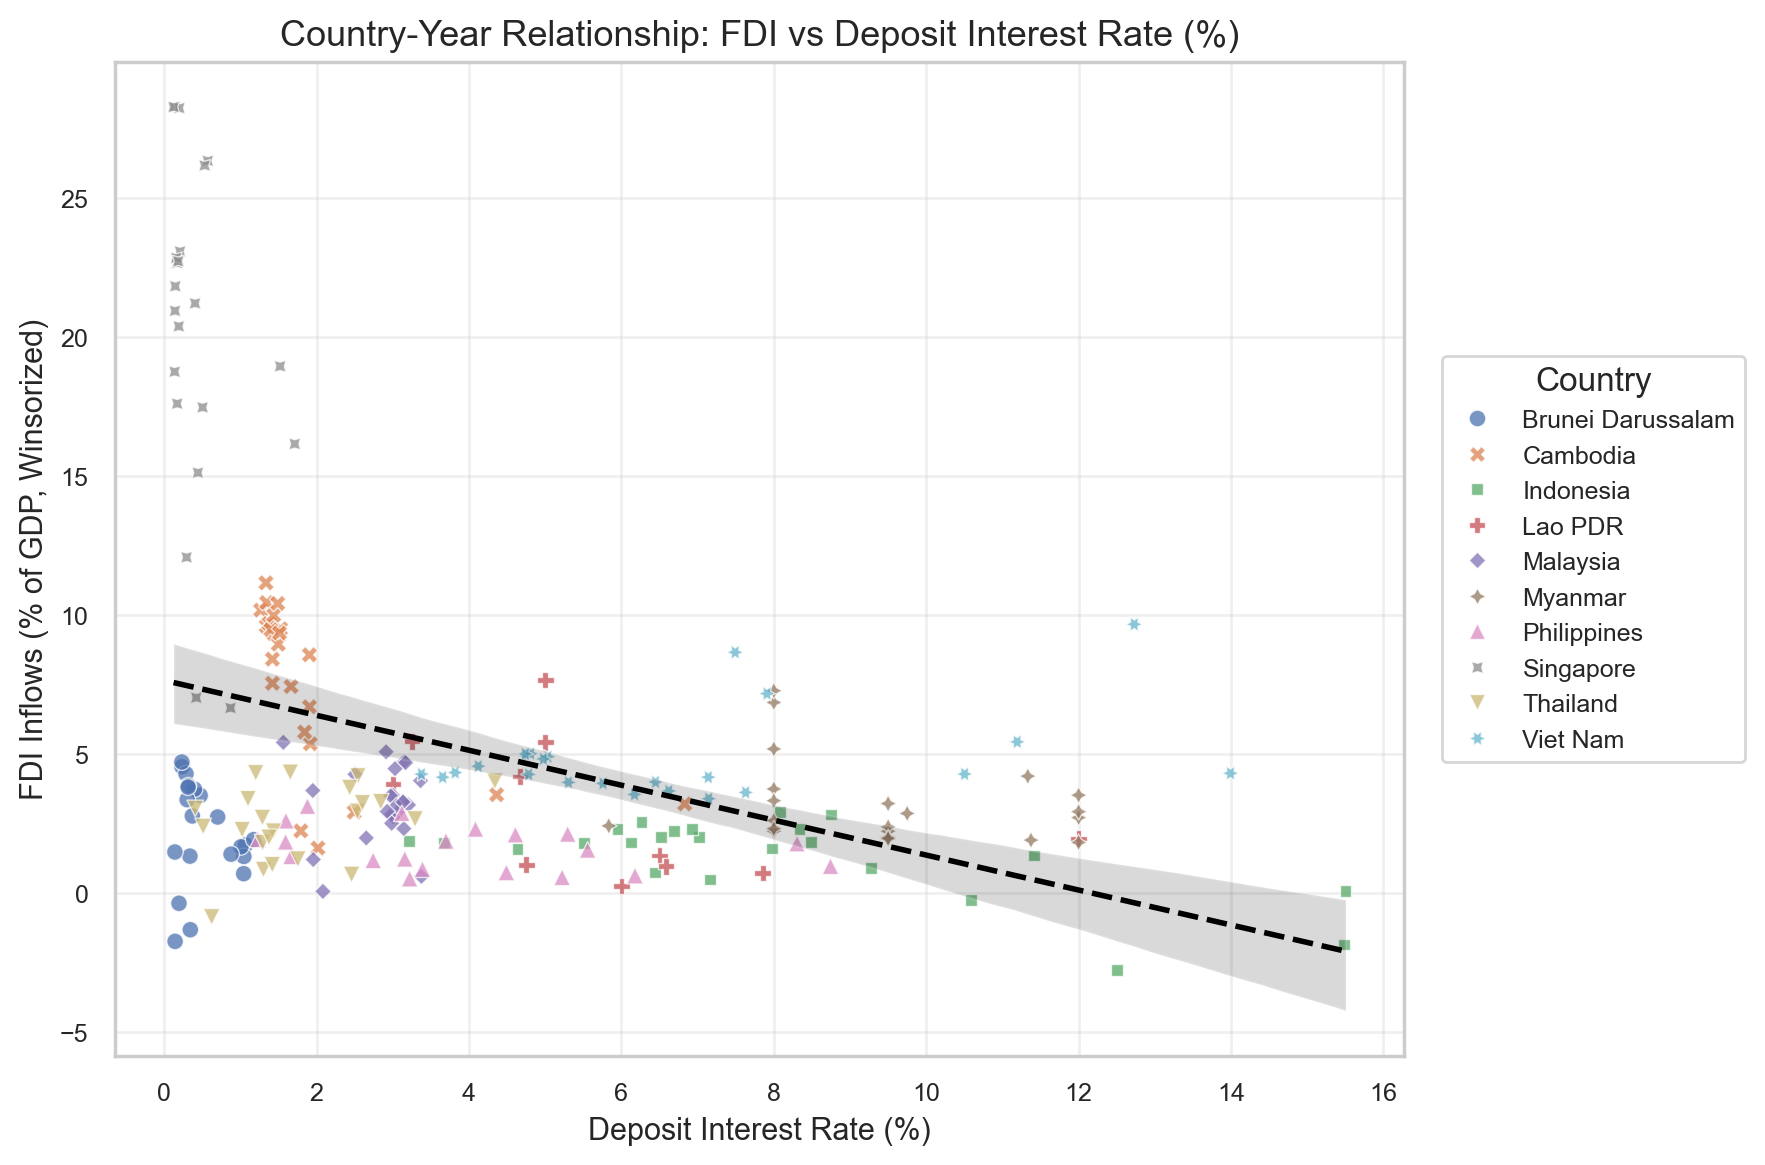
\includegraphics[width=0.75\textwidth]{assets/scatter_country_year_deposit_interest_fdi.png}
\caption{Deposit interest rate vs.\ FDI net inflows. A slight negative slope is visible in the raw data, but the association is overwhelmed by between-country heterogeneity once country fixed effects are included.}
\label{fig:bivariate-dep-fdi}
\end{figure}

\begin{figure}[htbp]
\centering
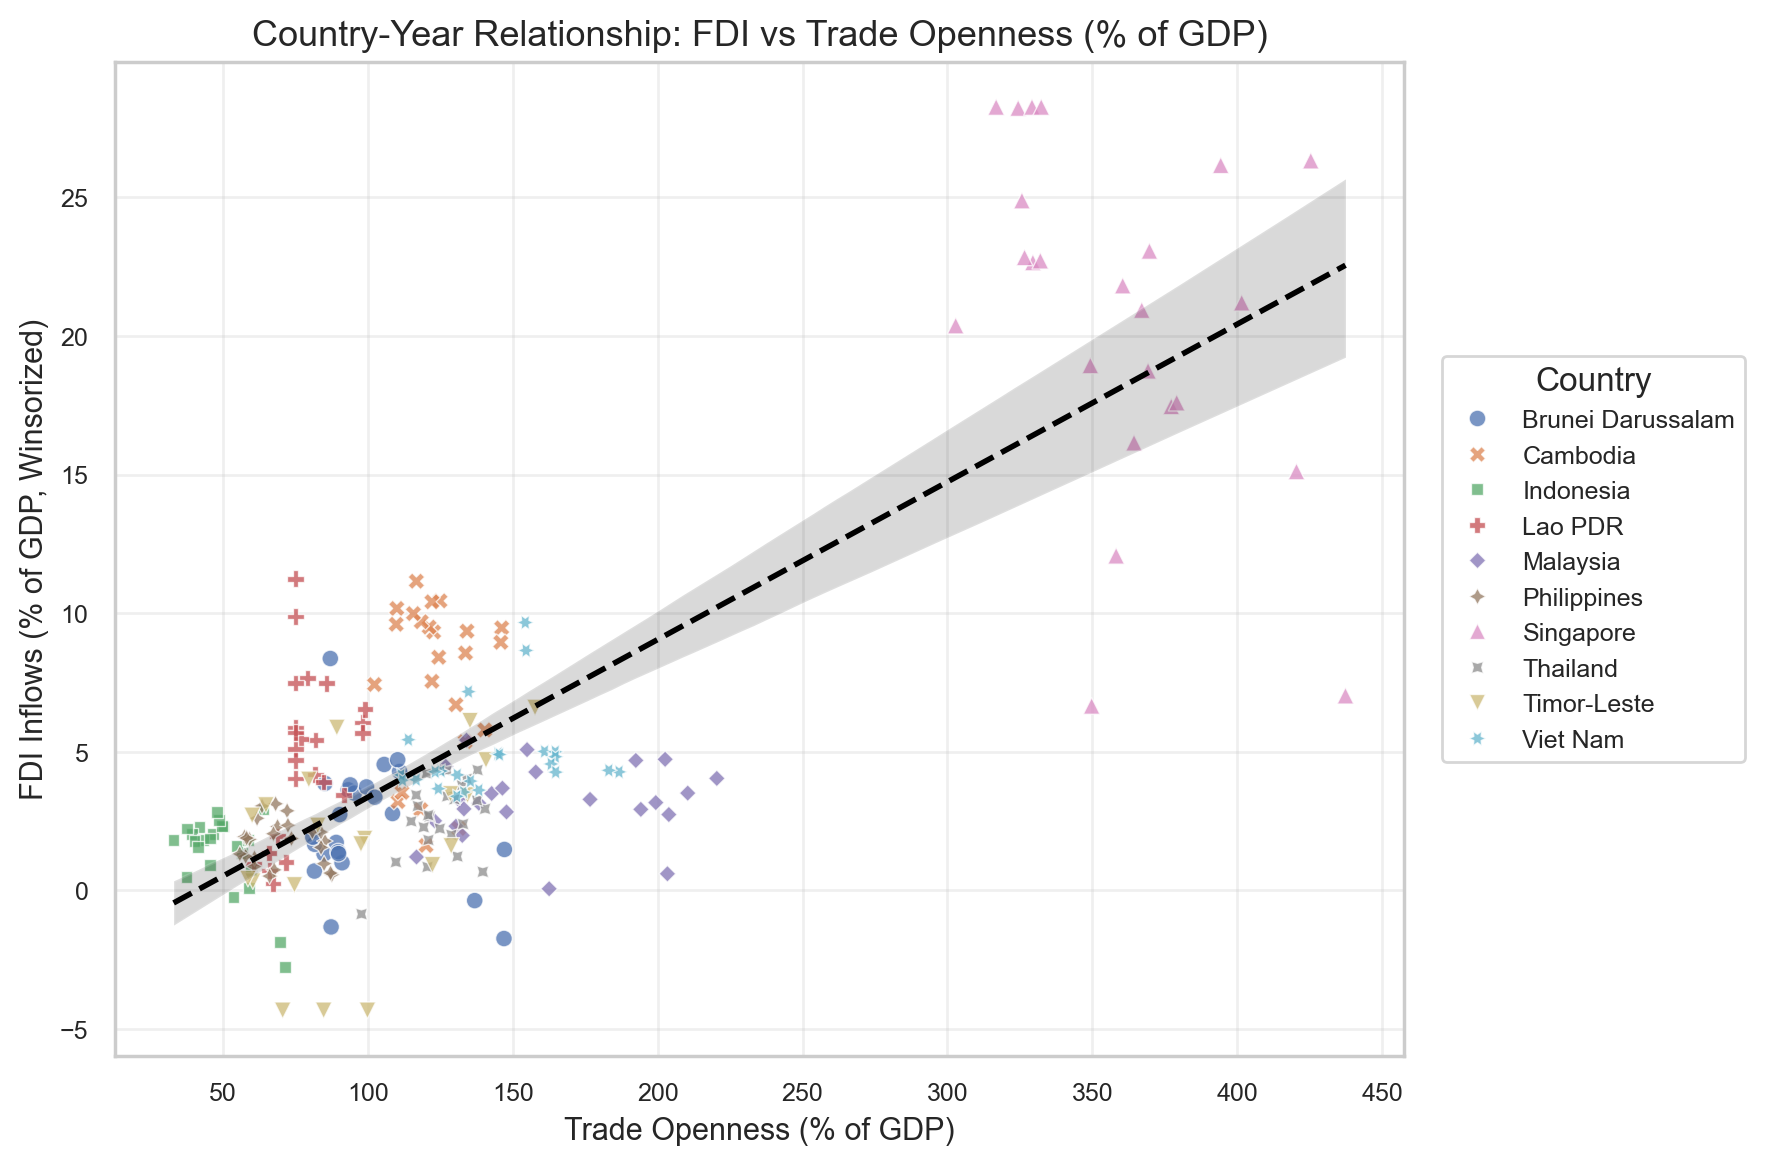
\includegraphics[width=0.75\textwidth]{assets/scatter_country_year_trade_fdi.png}
\caption{Trade openness vs.\ FDI net inflows. The strong positive unconditional correlation ($r=0.78$) is driven largely by Singapore; the within-country signal is weaker, consistent with the imprecise trade coefficients in the FE-DK regressions.}
\label{fig:bivariate-trade-fdi}
\end{figure}

\subsection{Correlations and Data Coverage}
\label{app:correlations-coverage}

\begin{figure}[htbp]
\centering
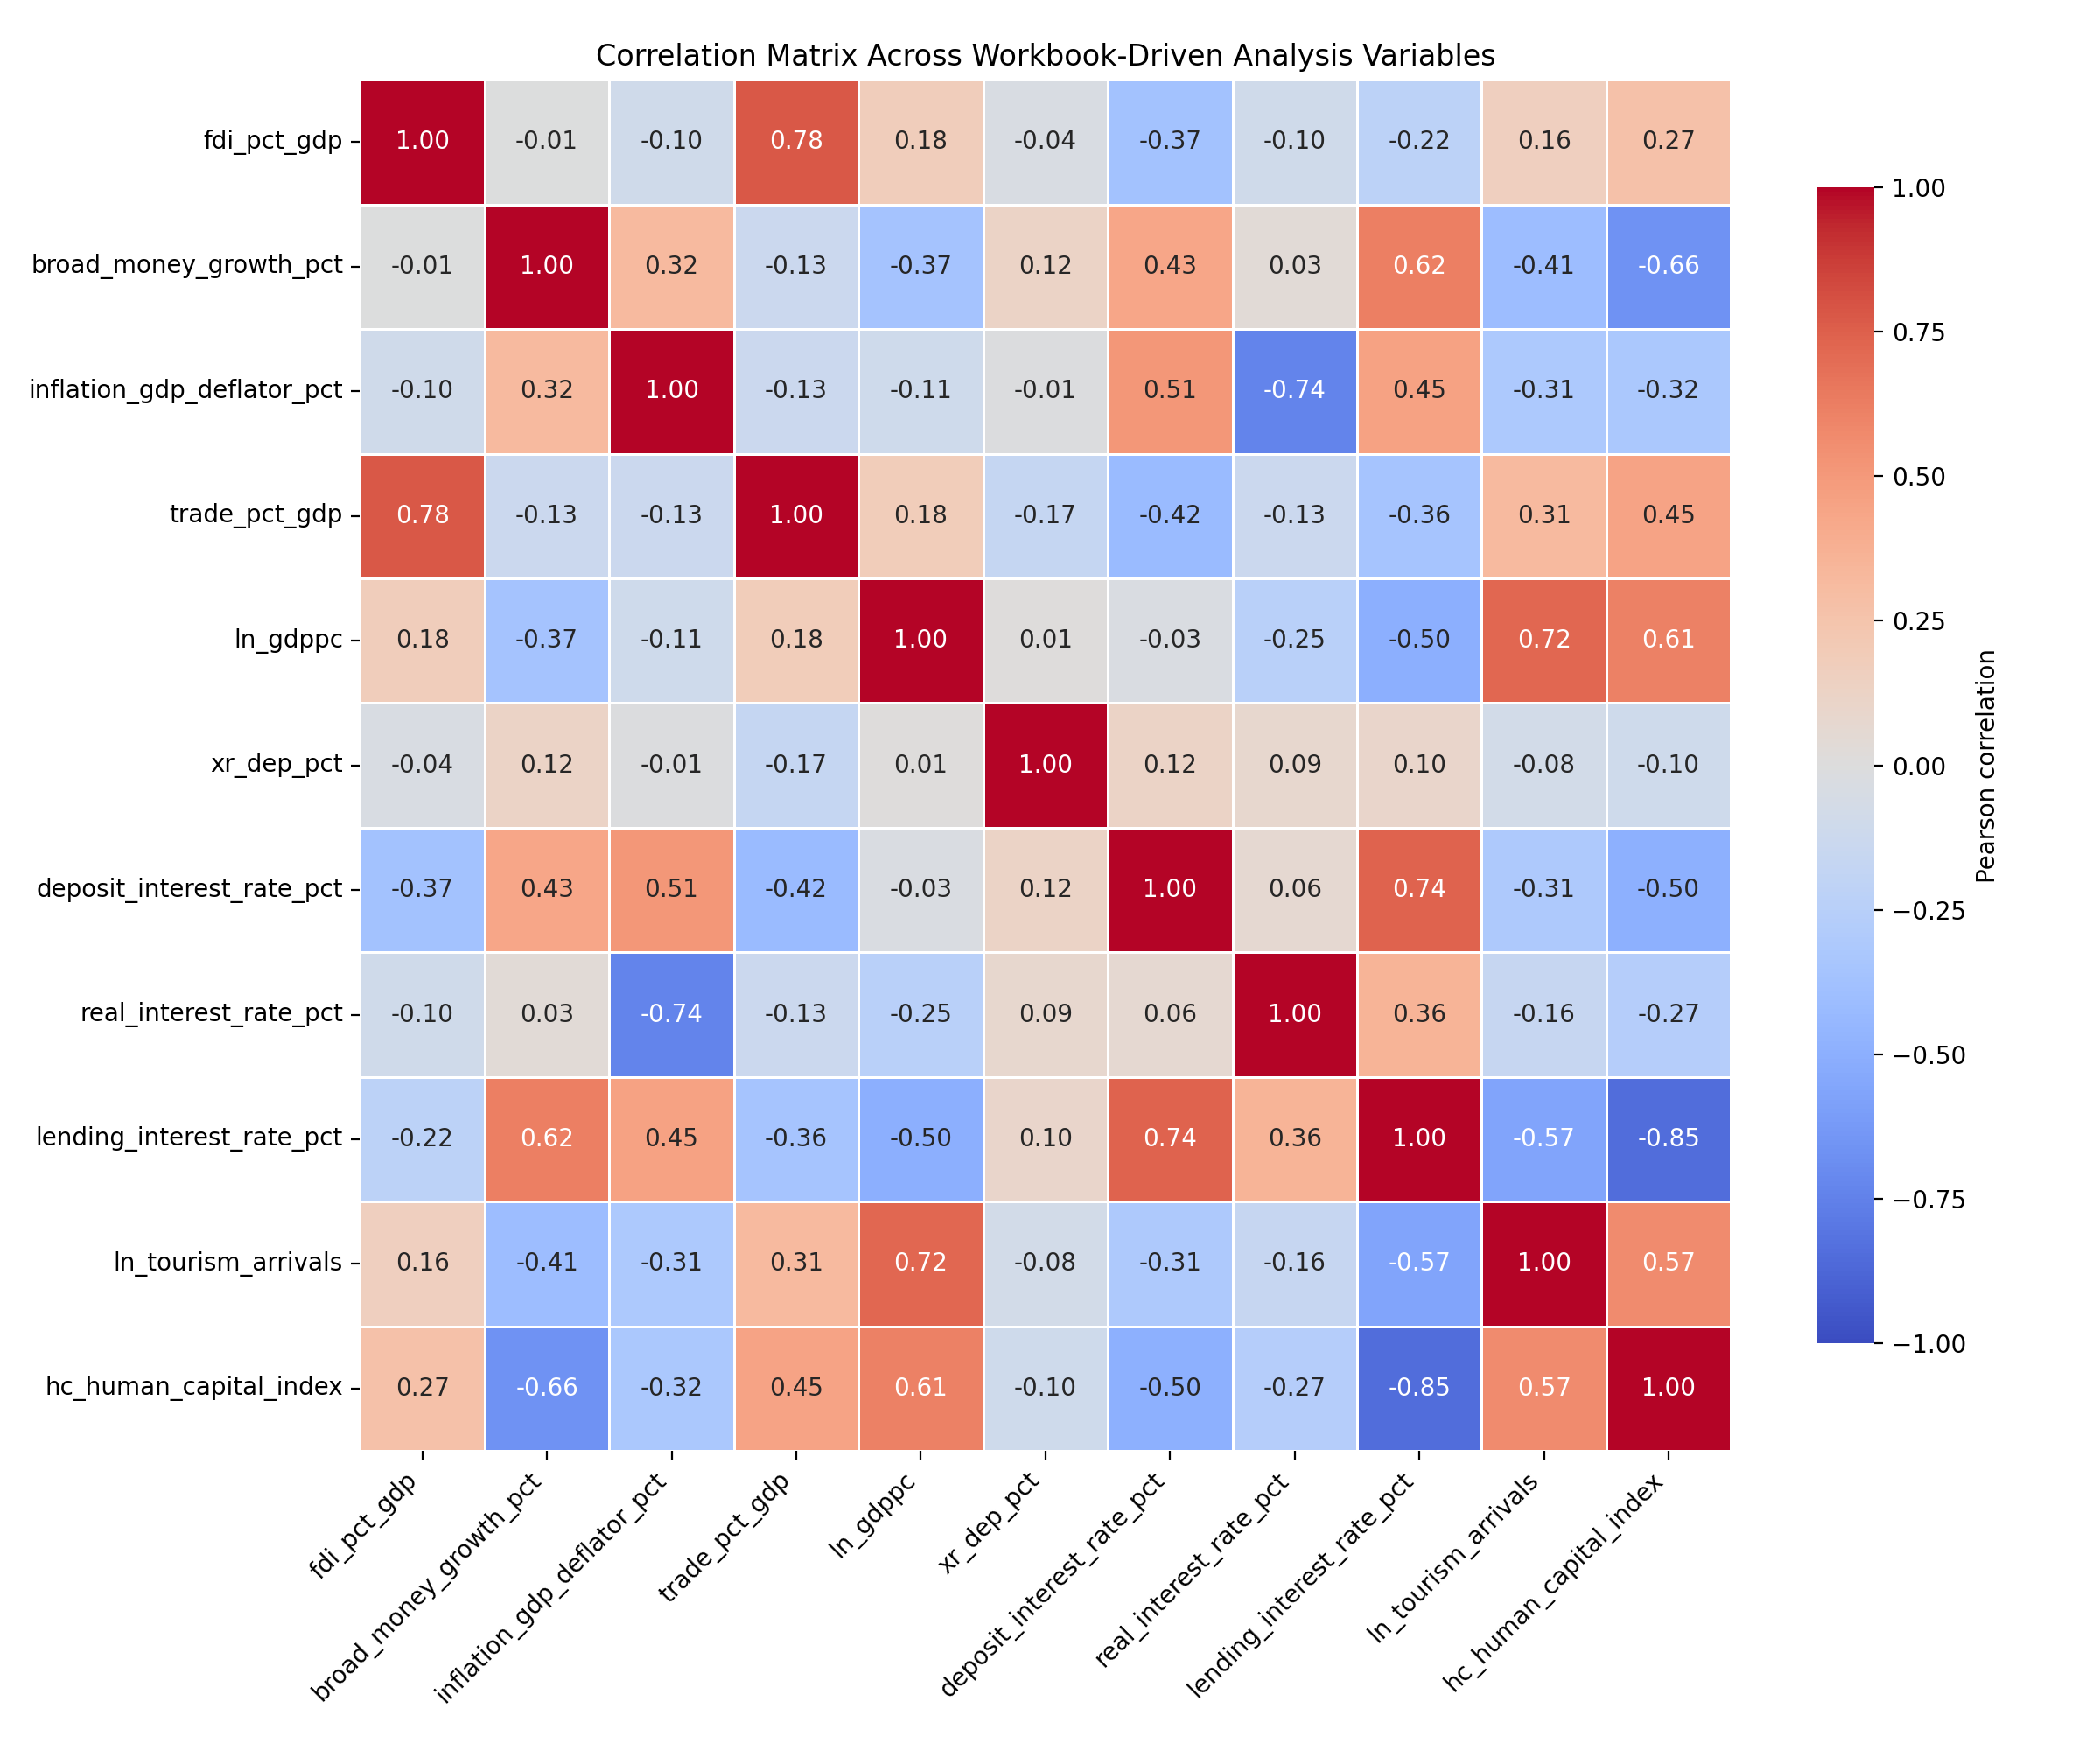
\includegraphics[width=\textwidth]{assets/correlation_matrix_main_variables.png}
\caption{Pearson correlation matrix of main analysis variables. FDI is positively correlated with trade openness (0.78) and GDP per capita, and negatively correlated with deposit ($-0.37$), real ($-0.10$), and lending ($-0.22$) interest rates. Broad money growth correlates positively with inflation (0.32) and negatively with the human capital index ($-0.67$).}
\label{fig:correlation-heatmap}
\end{figure}

\begin{figure}[htbp]
\centering
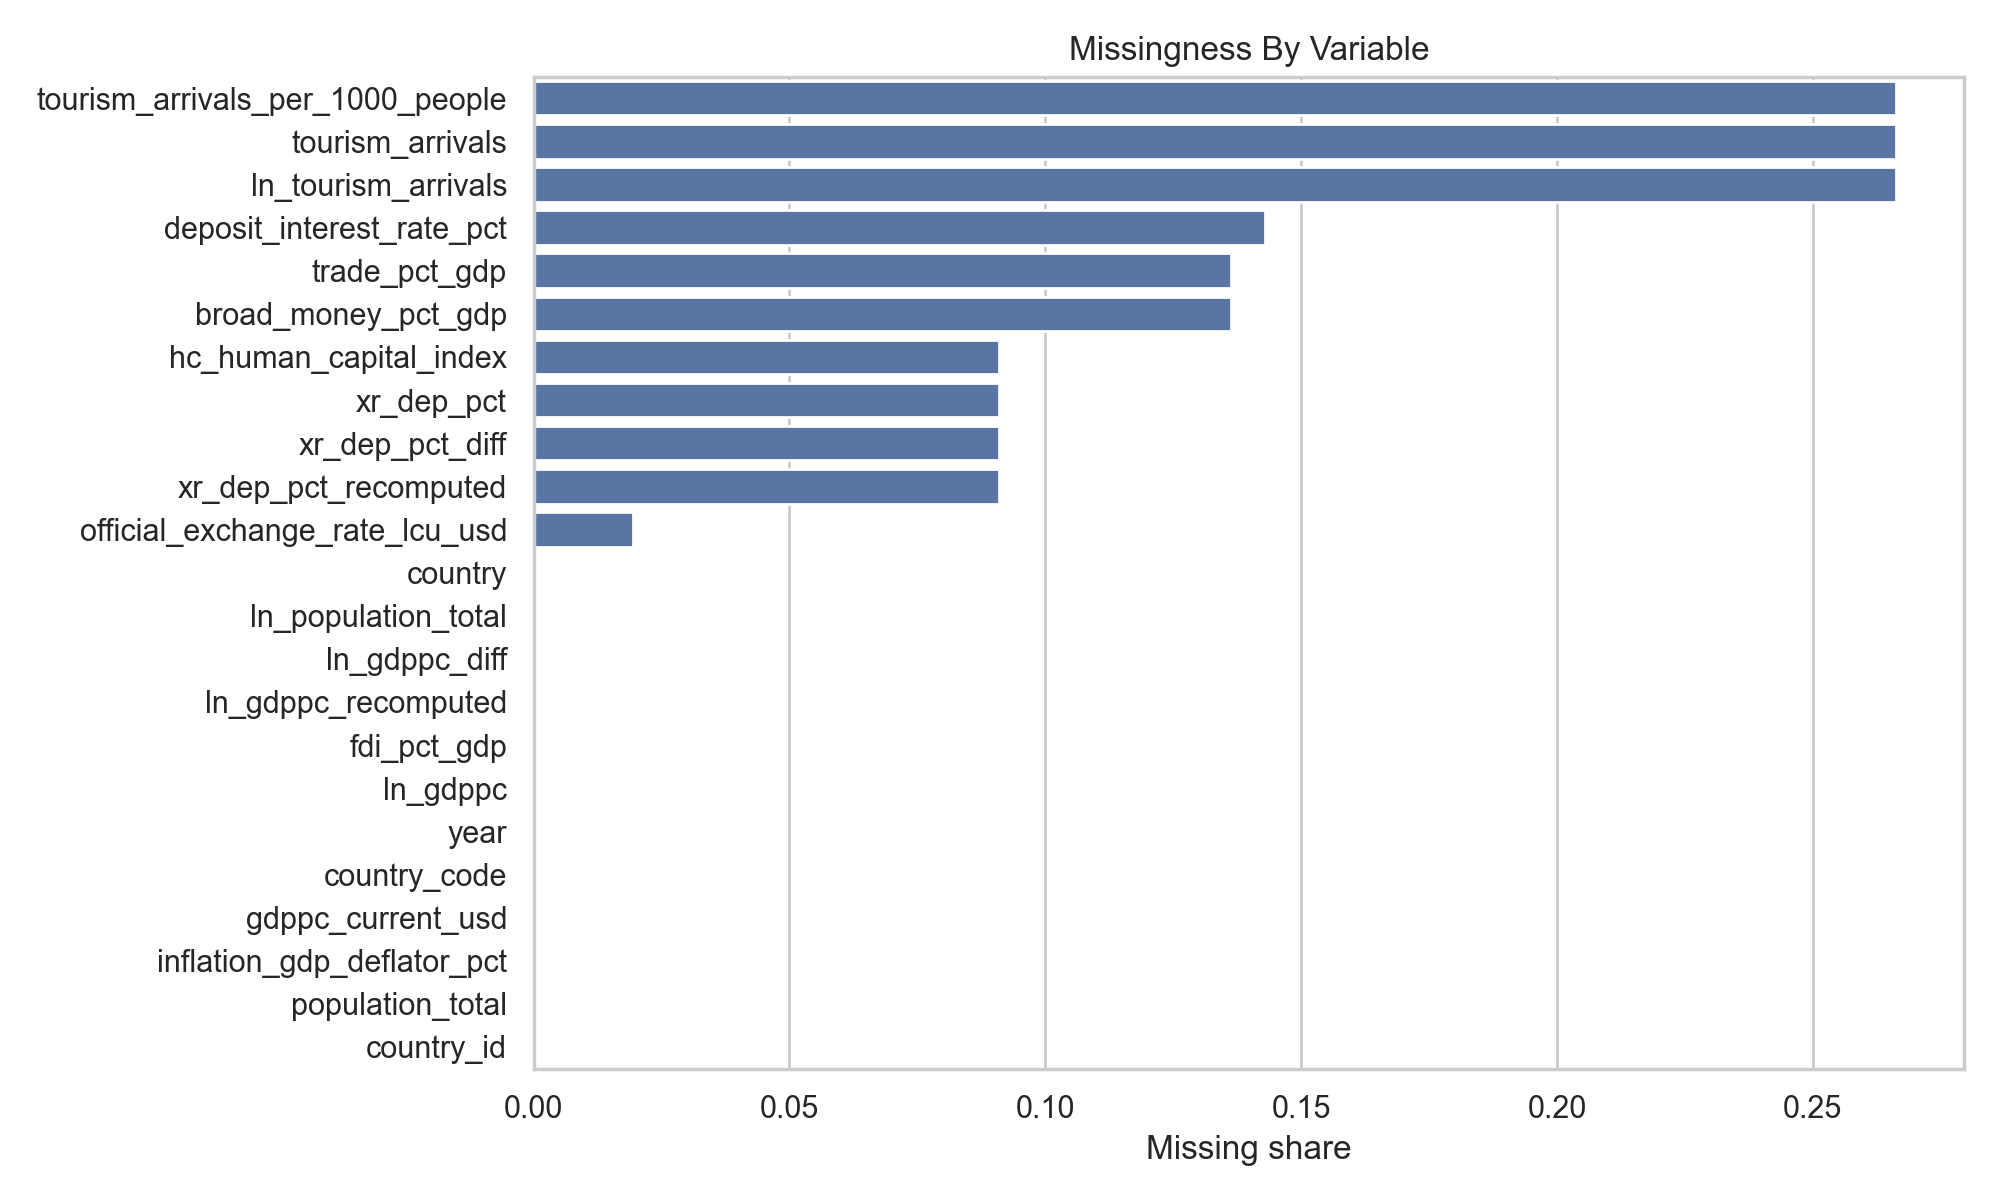
\includegraphics[width=0.8\textwidth]{assets/missingness_by_variable.png}
\caption{Missing data rates by variable. Interest-rate proxies have the highest missingness (19--27\%), concentrated in Cambodia, Lao PDR, and Timor-Leste. FDI and GDP per capita are fully observed. Controls have 0--9\% missingness.}
\label{fig:missingness}
\end{figure}
